\section{Interfejs graficzny}
W celu stworzenia GUI wykorzystano biblioteki \textit{Qt}. Interfejs graficzny zosta� zaprojektowany z wykorzystaniem programu \textit{QtDesigner}.

\subsection{Wykorzystane klasy}
Tworz�c interfejs wykorzystano biblioteki:

\begin{itemize}
\item \textbf{QGraphicsScene} - biblioteka pozwalaj�ca na stworzenie obiektu reprezentuj�cego dwuwymiarow� scen� graficzn�, na scenie mo�na tworzy� i umieszcza� obiekty (pojedyncze piksele, wieloboki), obiekty mo�na poddawa� transformacji przy pomocy klasy \textit{QTransform},
\item \textbf{QGraphicsView} - biblioteka, przy pomocy kt�rej mo�na wizualizowa� zawarto�� sceny utworzonej z wykorzystaniem klasy \textit{QGraphicsScene}.
 \end{itemize}

\subsection{Proponowany interfejs}
\begin{figure}[H]
  \centering
  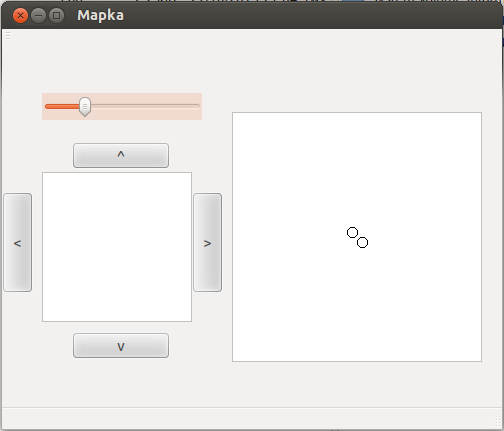
\includegraphics[width=0.5\textwidth]{img/okno.png}
\end{figure}
